\documentclass{ctexart}
\usepackage{amsmath}
\usepackage{float}
\usepackage{amssymb}
\usepackage{graphicx}
\usepackage{gbt7714}
\usepackage{pifont}
\usepackage{wrapfig}
\usepackage{multirow}
\usepackage{array}


\ctexset{
    % 修改 section。
    section={   
        name={,、},
        number={\chinese{section}}
    }
}

\title{密立根油滴实验}
\author{陆知辰-10225301478}
\date{\today}
\graphicspath{{figure/}}

\begin{document}

\begin{titlepage}
  \centering
  % 插入图片
  
\includegraphics[width=0.5\textwidth]{ecnu.png}
  
  % 空行用于调整标题位置
  \vspace*{\baselineskip}
  
  % 标题
  \Huge\textbf{物\quad 理\quad 实\quad 验 \quad (二)}
  % 空行用于调整标题和其他信息之间的间距
  \vspace*{0.3\baselineskip}
  
  % 具体实验名称
  \huge 密立根油滴实验
  
  % 空行用于调整时间和其他信息之间的间距
  \vspace*{2\baselineskip}
  
  % 时间
  \large 时间:\today
  
  % 空行用于调整时间和其他信息之间的间距
  \vspace*{\baselineskip}
  
  % 创作人
  \large 创作人:陆知辰
  
  % 空行用于调整创作人和学号之间的间距
  \vspace*{\baselineskip}
  
  % 学号
  \large 学号:10225301478
  
\end{titlepage}
\newpage
\tableofcontents
\newpage
\section{实验摘要}
  \subsection{实验概要}
  密立根油滴实验在近代物理学发展史上是一个十分重要的实验,它证明了任何带
  电体所带的电荷都是元电荷的整数倍,明确了电荷的不连续性,并精确地测定了元电荷的数值,
  为从实验上测定其他一些基本物理量提供了可能性。

  \subsection{实验目的}
  1.\quad 了解密立根油滴实验的设计思想。

  2.\quad 掌握带电油滴在重力场和静电场中运动的测量方法。
  
  3.\quad 掌握测量元电荷的数据处理方法。

\section{实验原理}
  \subsection{动态(非平衡)法测油滴电荷}
  一个质量为m、带电荷量为g的油滴处在两块平行极板之间,
  在平行极板未加电压时,油滴受重力作用而加速下降,由于空气阻力的作用,
  下降一段距离后,
  油滴将作匀速运动,速度为$v_{g}$,这时重力与阻力平衡(空气浮力忽略不计),
  如图\ref{shouli}所展示的那样。

  \begin{figure}[H]
    \centering
    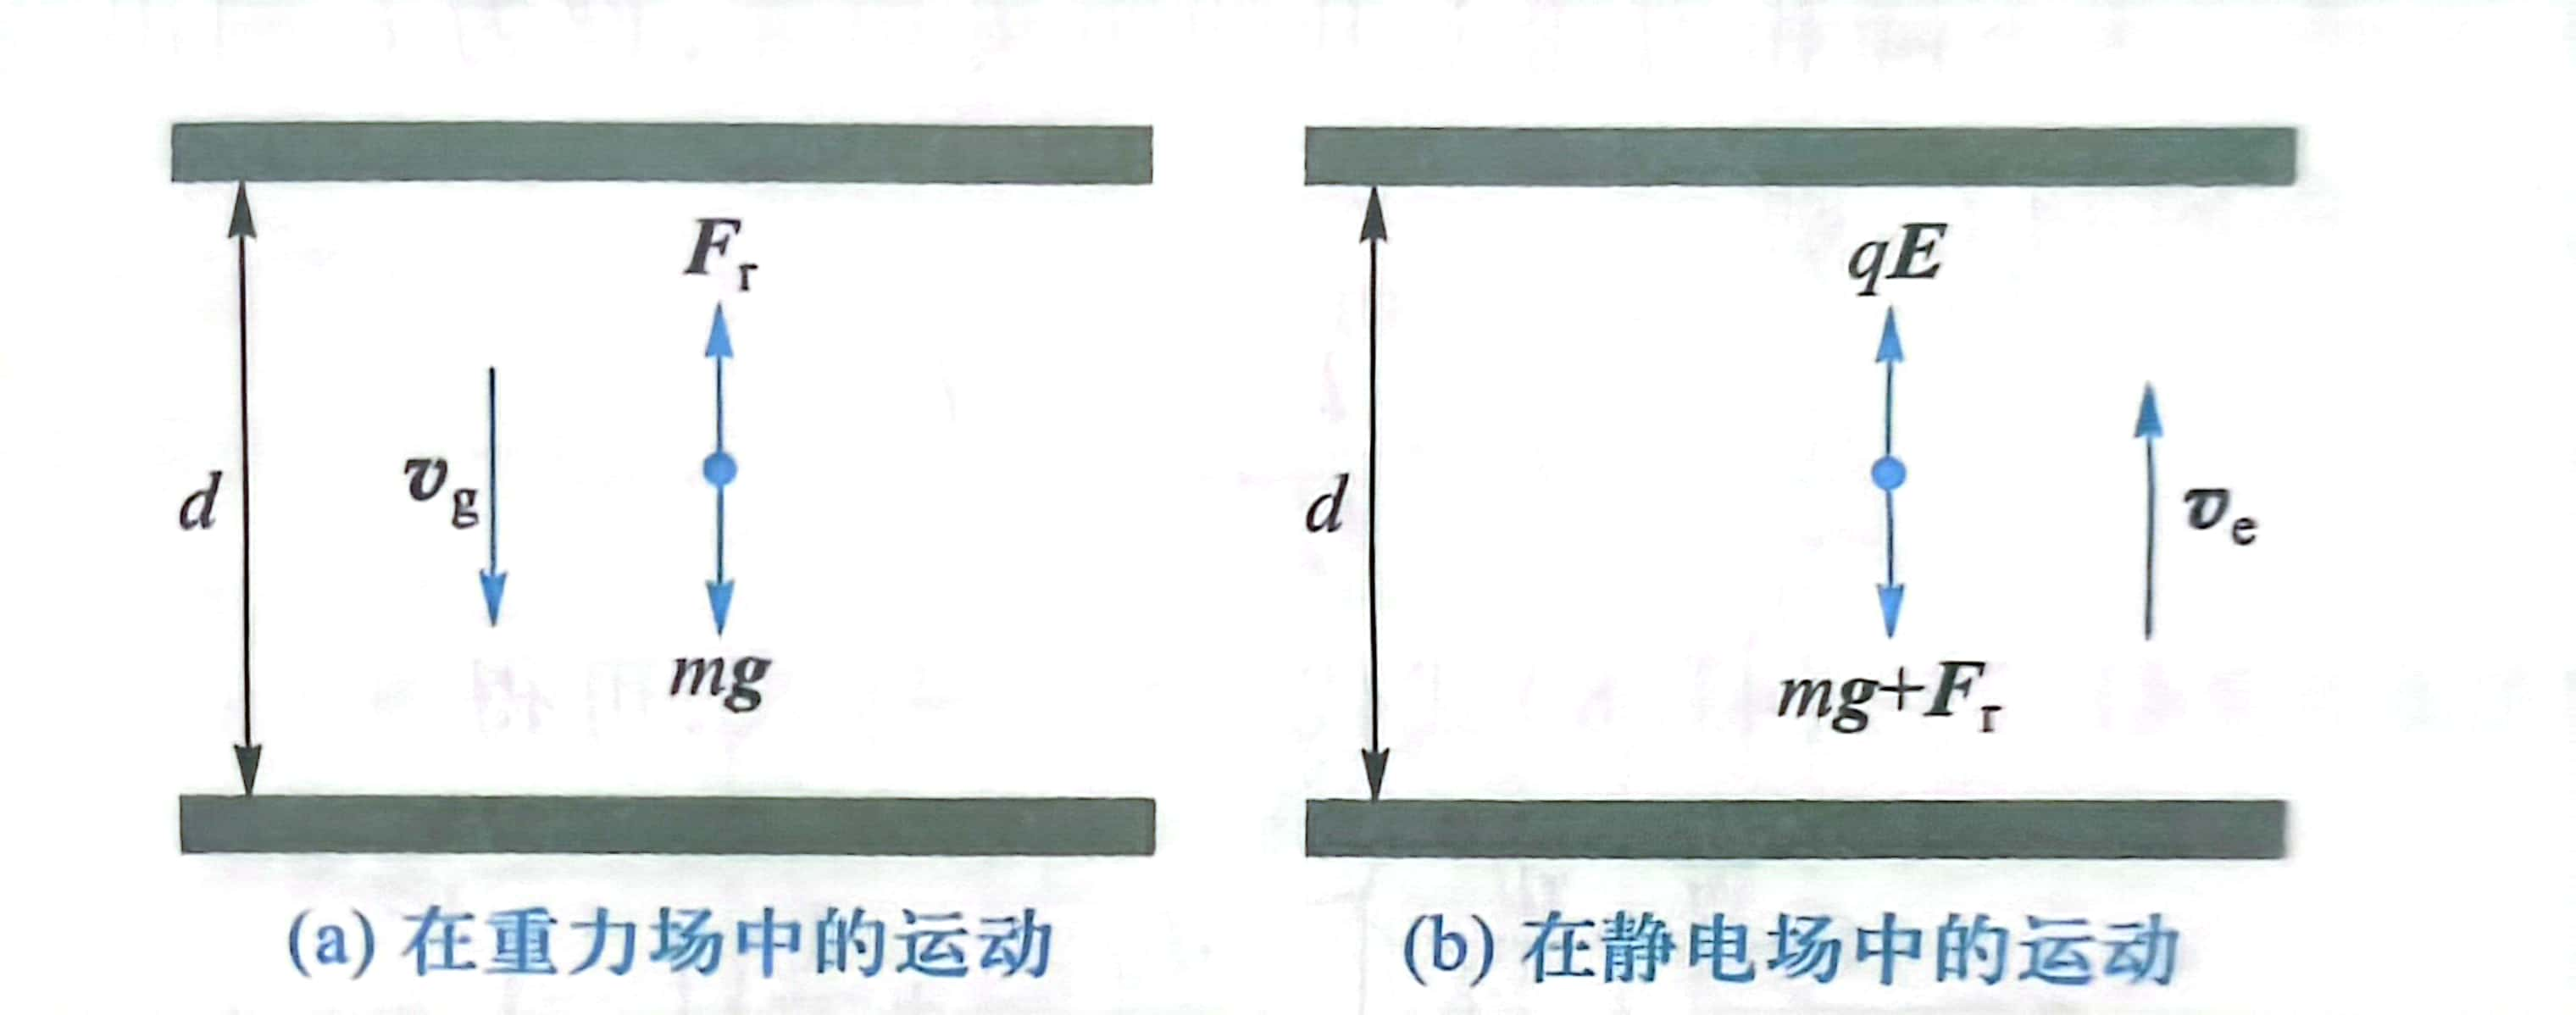
\includegraphics[height=0.6\textwidth,width=1\textwidth]{shouli.jpg}
    \caption{电荷在极板间运动时受力情况}\label{shouli}
  \end{figure}

  根据斯托克斯定律,黏性力为

  \begin{equation}
    F_{r}=6 \pi a \eta v_{g}
  \end{equation}

  式中$\eta$是空气的黏度,a是油滴的半径,这时有

  \begin{equation}
    6 \pi a \eta v_{g} = m g
  \end{equation}

  当在平行极板上加电压U时,油滴处在场强为E的静电场中,
  设电场力qE与重力方向相反,
  使油滴受电场力加速上升,由于空气阻力作用,上升一段距离后,油滴所受的空气阻力、
  重力与电场力达到平衡(空气浮力忽略不计),则油滴将匀速上升,此时速度为$v_{e}$,则有

  \begin{equation}
    6 \pi a \eta v_{e} = qE - mg
  \end{equation}

  根据$E = \frac{U}{d}$ 结合上文的结论可以得到

  \begin{equation}
    q = mg (\frac{d}{U}) (\frac{v_{g}+v_{e}}{v_{g}})
  \end{equation}

  为测定油滴所带电荷量q、除应测出U、d和速度$v_{e}$和$v_{g}$。外,
  还须知油滴质量m.由于空气中悬浮和表面张力作用,可将油滴看作圆球,其质量为

  \begin{equation}
    m = \frac{4}{3} \pi a^{3} \rho
  \end{equation}

  其中$\rho$为油滴的密度。最终可以得到邮递的半径为

  \begin{equation}
    a = ( \frac{9\eta v_{g}}{2\rho g} )^{\frac{1}{2}}
  \end{equation}

  考虑到油滴非常小,空气 已不能看作连续介质,空气的粘度$\eta$应该修正为:
  
  \begin{equation}
    \eta^{'} = \frac{\eta}{1+ \frac{b}{pa} }
  \end{equation}

  式中b为修正常数,p为空气压强,a为未经修正过的油滴半径,由于它在修正项
  中,所以不必计算得很精确。
  实验时取油滴匀速下降和匀速上升的距离相等,设为l,测出油滴匀速下降的时间$t_{g}$,匀速上升的时间$t_{e}$。则
  
  \begin{equation}
    v_{g} = \frac{l}{t_{g}} \quad v_{e}=\frac{l}{v_{e}}
  \end{equation}

  最终可以得到

  \begin{equation}
    q = \frac{18\pi}{\sqrt{2\rho g}} (\frac{\eta l}{1+ \frac{b}{pa} })^{\frac{3}{2}} \frac{d}{U} (\frac{1}{t_{e}} + \frac{1}{t_{g}}) (\frac{1}{t_{g}})^{\frac{1}{2}}
  \end{equation}

  令

  \begin{equation}
    K = \frac{18\pi d}{\sqrt{2\rho g}} (\frac{\eta l}{1+ \frac{b}{pa} })^{\frac{3}{2}}
  \end{equation}

  可以得到

  \begin{equation}
    q = K (\frac{1}{t_{e}} + \frac{1}{t_{g}}) (\frac{1}{t_{g}})^{\frac{1}{2}} / U
  \end{equation}

  此公式即为动态(非平衡)法测油滴电荷的公式

  \subsection{静态(平衡)法测油滴电荷}
  调节平行板之间的电压,使油滴不动,$v_{e} = 0$,即 $t \rightarrow \infty $,有

  \begin{equation}
    q = K (\frac{1}{t_{g}})^{\frac{3}{2}} \frac{1}{U}
  \end{equation}

  或者

  \begin{equation}
    q = \frac{18\pi}{\sqrt{2\rho g}} (\frac{\eta l}{t_{g}(1+ \frac{b}{pa}) })^{\frac{3}{2}} \frac{d}{U}
  \end{equation}

  上式即为静态发测油滴电荷的公式。

  为了求电子电荷量,对实验测得的各个电荷q求出的最大公约数,就是元电荷e的值,也就是电子电荷量的绝对值。

\section{实验装置器材介绍}
密立根油滴仪(包含油滴盒、油滴照明装置、调平系统、测量显微系统、供电电源、电子停表及喷雾器等),显示器,油滴管等。

油滴盒的结构如图\ref{jiegou}所示.它由两块经过精磨的金属平板,中间垫以胶木圆环,
构成的平行板电容器组成.在上板中心处有油雾孔,使微小油滴可以进入电容器中间的电场空间,胶术圆环上有进光孔和观察孔。
进入电场空间内的油滴由照明装置照明,油滴盒可通过调平螺丝调整水平,用水准仪检查水平情况,
油滴盒防风罩前装有测量显微镜,用来观察油滴,在目镜头中装有分划板.

\begin{figure}[H]
  \centering
  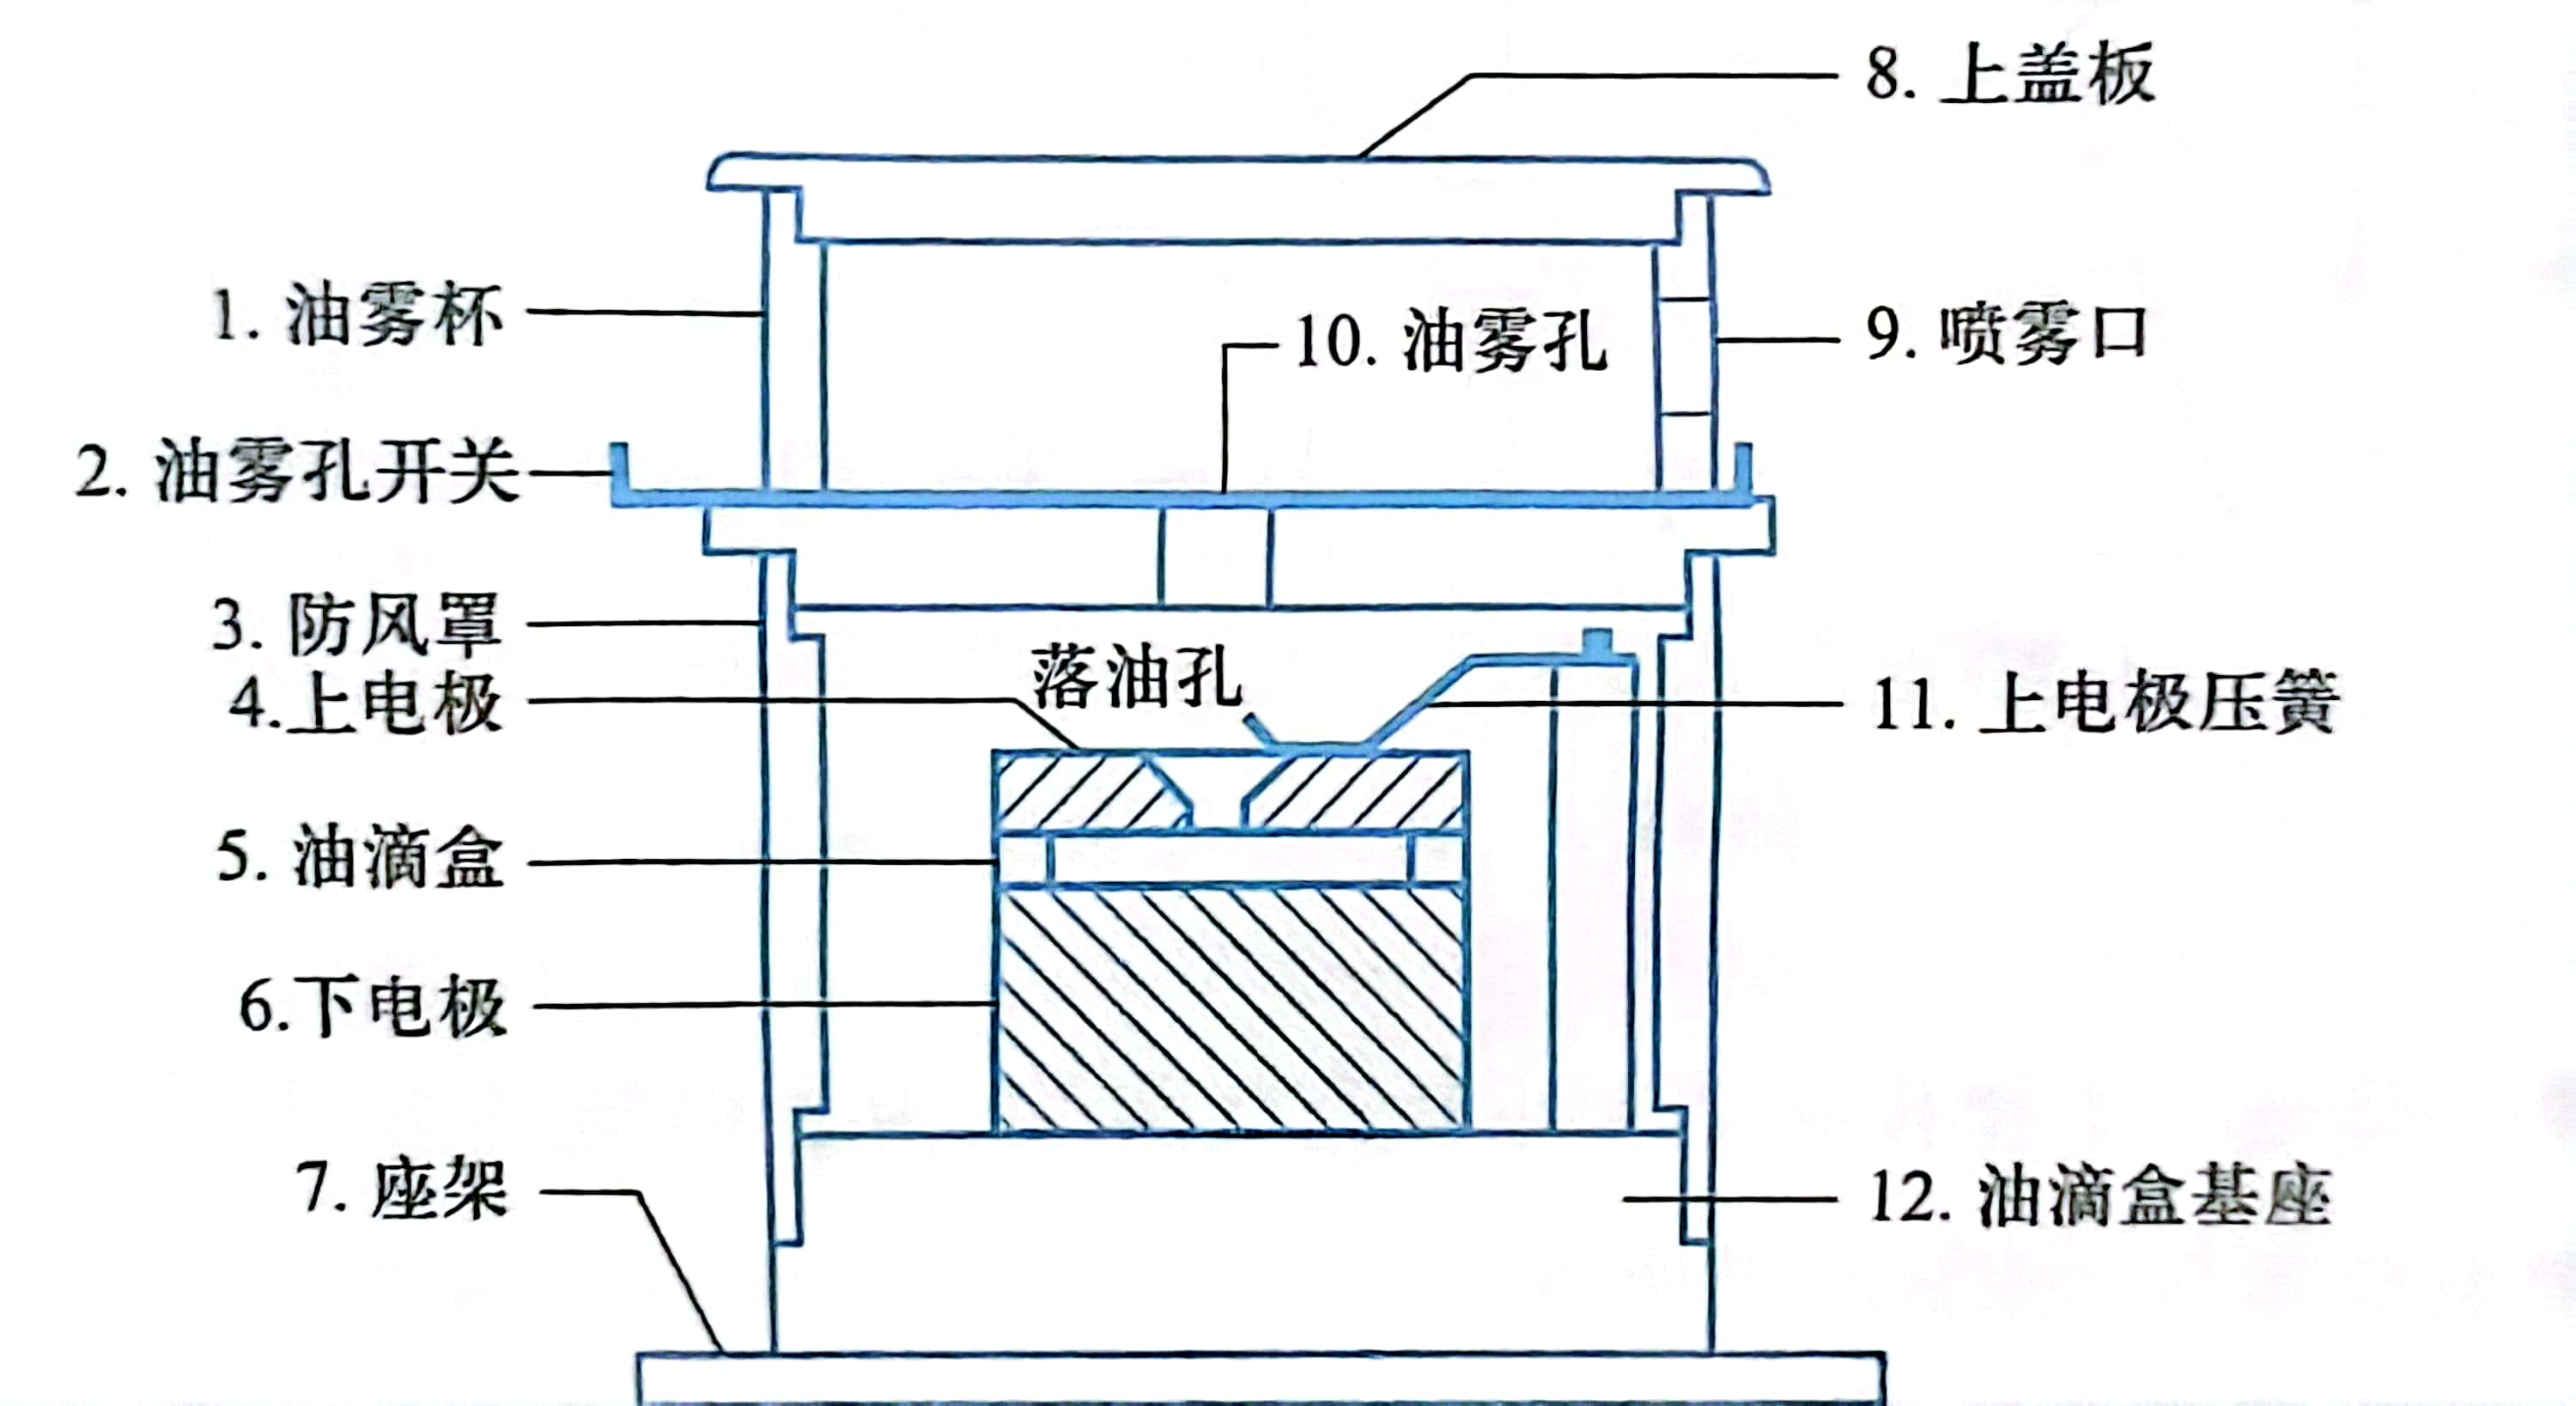
\includegraphics[height=0.7\textwidth,width=1\textwidth]{yiqijiegou.jpg}
  \caption{密立根实验仪器结构示意图}\label{jiegou}
\end{figure}

密立根油滴仪所具有的各个部分的功能如下:

电源开关:打开/关闭电源,控制平衡电压、提升电压和计时器,当电源关闭时,开关的指示灯为暗,打开电源,电源指示灯变亮。

水平调节仪:调节密立根油滴仪和桌面的水平情况,对水平调节仪的底座旋钮进行调节,
使水平调节仪的水平气泡处在中央位置,如果水平气泡不在中央位置,则会影响油滴下落的观察和上升时间的计量。

油滴管:喷出雾状油滴。

显微镜:调节显示器上油滴的清晰程度。

平衡电压挡:控制电压的正负极以及数值。

提升电压挡:在平衡电压数值的绝对值之上加上一定电压。

计时器:记录油滴的上升和下落的时间。

平衡电压旋钮:微调电压的数值。

\begin{figure}[H]
  \centering
  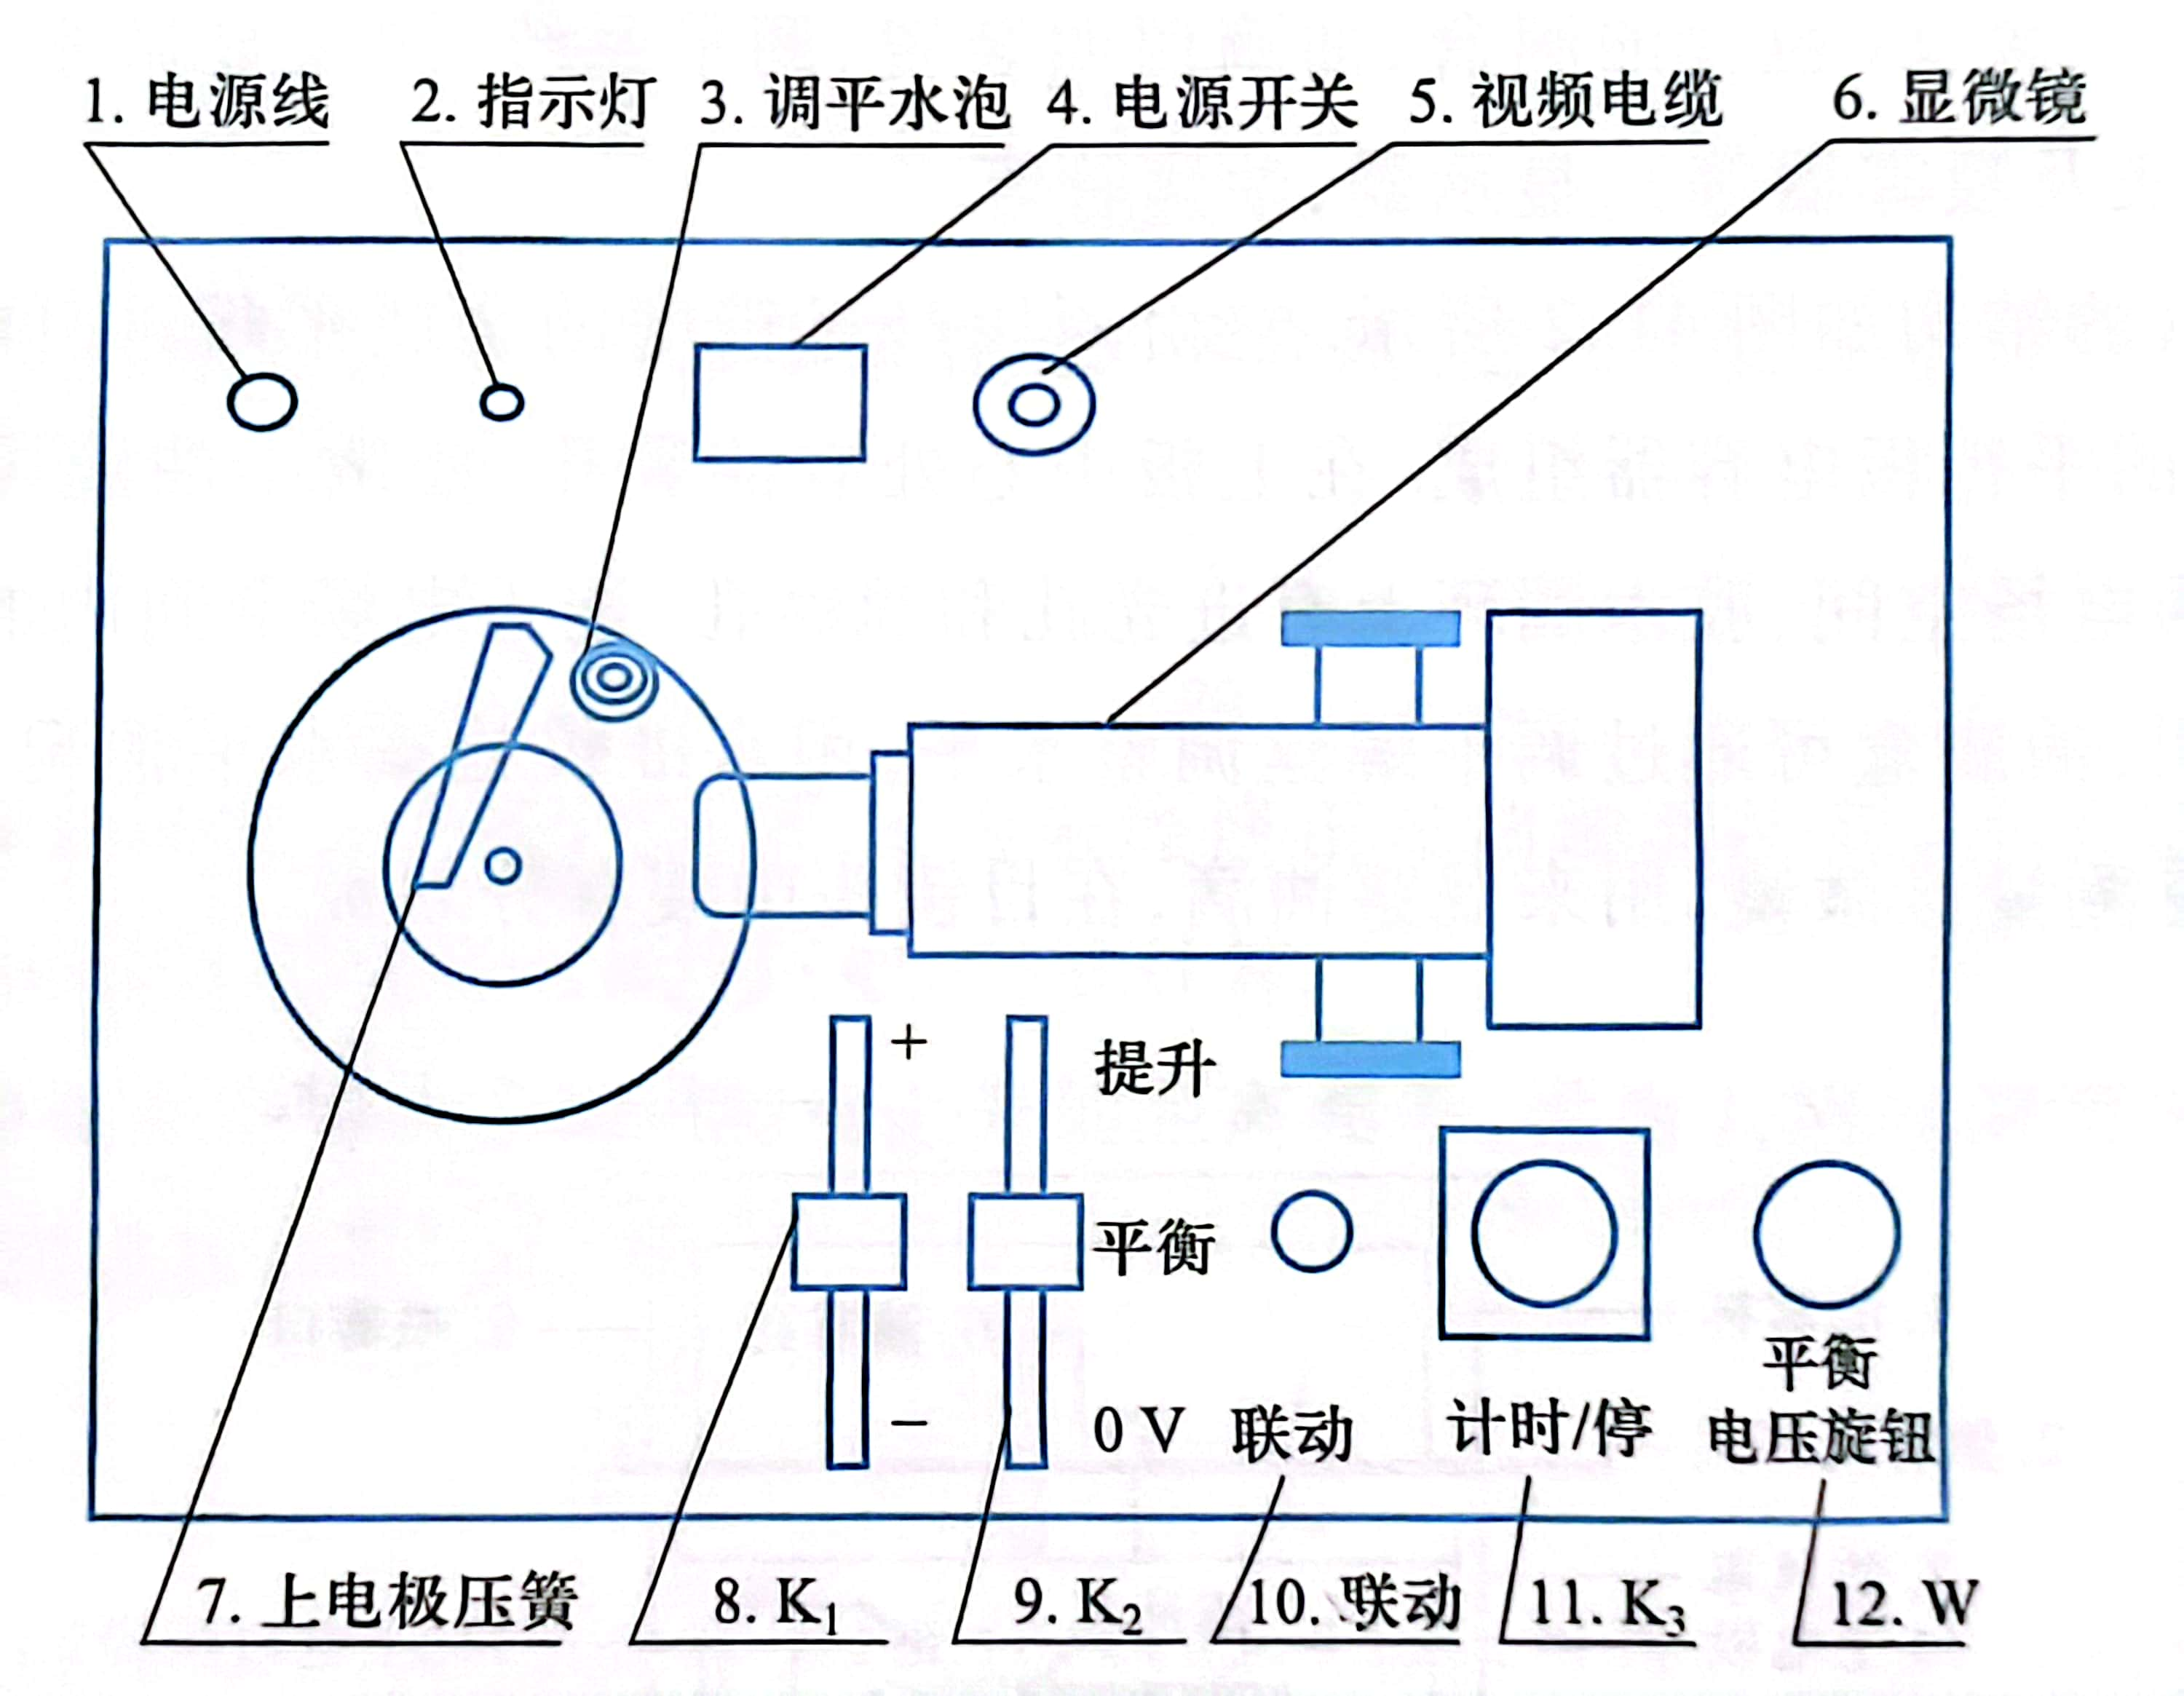
\includegraphics[height=0.7\textwidth,width=1\textwidth]{caozuopan.jpg}
  \caption{密立根实验仪器操作盘}\label{caozuopan}
\end{figure}

其控制面板如图\ref{caozuopan}所示.电容器极板上所加电压由直流平衡电压和直流升降电压两部分组成。
其中平衡电压大小连续可调,并可从显示屏上直接读数,其极性由换向开关控制,以满足对不同极性电压的需要,
升降电压的大小可连续调节,并可通过换向开关叠加在平衡电压上,以控制油滴在电容器内上下的位置。

油滴实验是一个操作技巧要求较高的实验,为了得到满意的实验结果,必须仔细认真调整油滴仪.调节过程如下:

\noindent(1)首先要调节调平螺丝,将平行电极板调到水平,使平衡电场方向与重力方向平行以免引起实验误差。

\noindent(2)调节显微镜焦点,使油滴清晰显示在显示器上。

\noindent(3)唢雾器是用来快速向油滴仪内喷油雾的,在喷射过程中,由于摩擦作用可使油滴带电。

当油雾从唢雾口喷人油滴室内后,视场中将出现大量清晰的油滴,犹如夜空繁星.试加上平衡电压,
改变其大小和极性,驱散不需要的油滴,练习控制其中一颗油滴的运动,并记录油滴经过两条横丝间距所用的时间。
\newpage

\section{实验内容及实验步骤}
  \subsection{讲仪器调整至待测状态}
  调节仪器底座上的三只调平手轮,将水泡调平,调节显微镜简前端使其和底座前端对齐,喷油后再稍稍前后微调即可.在使用中,前后调焦范围不要过大,取前后调焦1mm内的油滴较好。

  打开监视器和油滴仪的电源,进人测量状态后,显示出标准分划板刻度线及电压值U、下落时间t。

  \subsection{测量练习}
    \subsubsection{选择油滴}
    选择一颗合适的油滴十分重要,大而亮的油滴必然质量大,所带电荷也多,而匀速下降时间却很短,
    这增大了测量误差,给数据处理带来困难.我们通常选择平衡电压为200~300 V,匀速下落1.5 mm(6格)所用时间在8~20s的油滴较适宜。

    \subsubsection{平衡判断}
    判断油滴是否平衡要有足够的耐性。

    \subsubsection{记录时间}
    测准油滴上升或下降某段距离所需的时间,一是要统一油滴到达刻度线什么位置才认为油滴已踏线;二是眼睛要平视刻度线,不要有夹角。

  \subsection{平衡法(静态法)测量}
  可将已调平衡的油滴用平衡电压开关控制移到“起跑”线上(一般取第2格上线),
  按计时开关,让计时器停止计时(值不必要为0),然后将平衡电压开关K,拨向“0V”,
  油滴开始匀速下降的同时,计时器开始计时。到“终点”(一般取第7格下线)时迅速将平衡电压开关K2拨向“平衡”,油滴立即静止,
  计时也立即停止,此时电压值和下落时间值显示在屏幕上,进行相应的数据处理即可。

  \subsection{动态法测量}
  分别测出加电压时油滴上升的速度和不加电压时油滴下落的速度,代入相应公式,
  求出e值,此时最好将平衡电压开关与计时开关联动断开,油滴的运动距离一般取1~1.5mm。
  选择10~20颗油滴,对某颗油滴重复测量5~10次,求得电子电荷量的平均值。
  在每次测量时都要检查和调整平衡电压,以减小偶然误差,避免因油滴挥发而使平衡电压发生变化。

  \subsection{数据处理}
    \subsubsection{数据处理用到的参量}
    \begin{table}[H]
      \centering
      \begin{tabular}{|c|c|}
        \hline
        \textbf{参量} & \textbf{量值} \\
        \hline
        油的密度 & $\rho = 981 kg \cdot m^{-3} (20 ^{\circ} C)$ \\
        \hline
        油滴匀速下降距离 & $l = 1.5 \times 10^{-3} m $ \\
        \hline
        修正常数 & $b = 6.17 \times 10^{-6} m \cdot cmHg$ \\
        \hline
        \multirow{2}{*}{大气压强} & $p = 76.0 cmHg$ \\
                                & (实际大气压可由气压表读出) \\
        \hline
        平行极板间距离 & $d = 5.00 \times 10^{-3} m$ \\
        \hline
      \end{tabular}
      \caption{数据处理可能用到的参量数据表}
      \label{tab:mytable}
    \end{table}
    
    \subsubsection{数据处理方法介绍}
    \ding{172}求最大公约数

    计算出各油滴的电荷后,求它们的最大公约数,即得元电荷e值

    \ding{173}倒过来验证法

    以元电荷的公认值为最大公约数去除测得的油滴的电荷量,
    得到一组接近于整数的值之后取整数,从而验证电荷的不连续性,
    用每一个测得的电荷量数值除去整数值得到每一个实验所测得的元电荷e的数值,
    再对所有的实验元电荷e值取平均值即可得到e的实验值。
    该方法优点是可以快速处理数据,缺点是颠倒了因果关系,不利于培养探索精神。

    \ding{174}作图法

    设实验得到m个油滴的带电荷量分别为$q_{1},q_{2},\cdots q_{m}$。
    由于电荷的量子化特性,应有$q_{i} = n_{i} e$,此为一直线方程,n为自变量,q为因变量,e为斜率。
    因此m个油滴对应的数据在 n-q坐标中将在同一条过原点的直线上,若找到满足这一关系的直线,就可用斜率求得e值.
    将e的实验值与公认值比较,求相对误差。

\section{实验原始数据}
\begin{figure}[H]
  \centering
  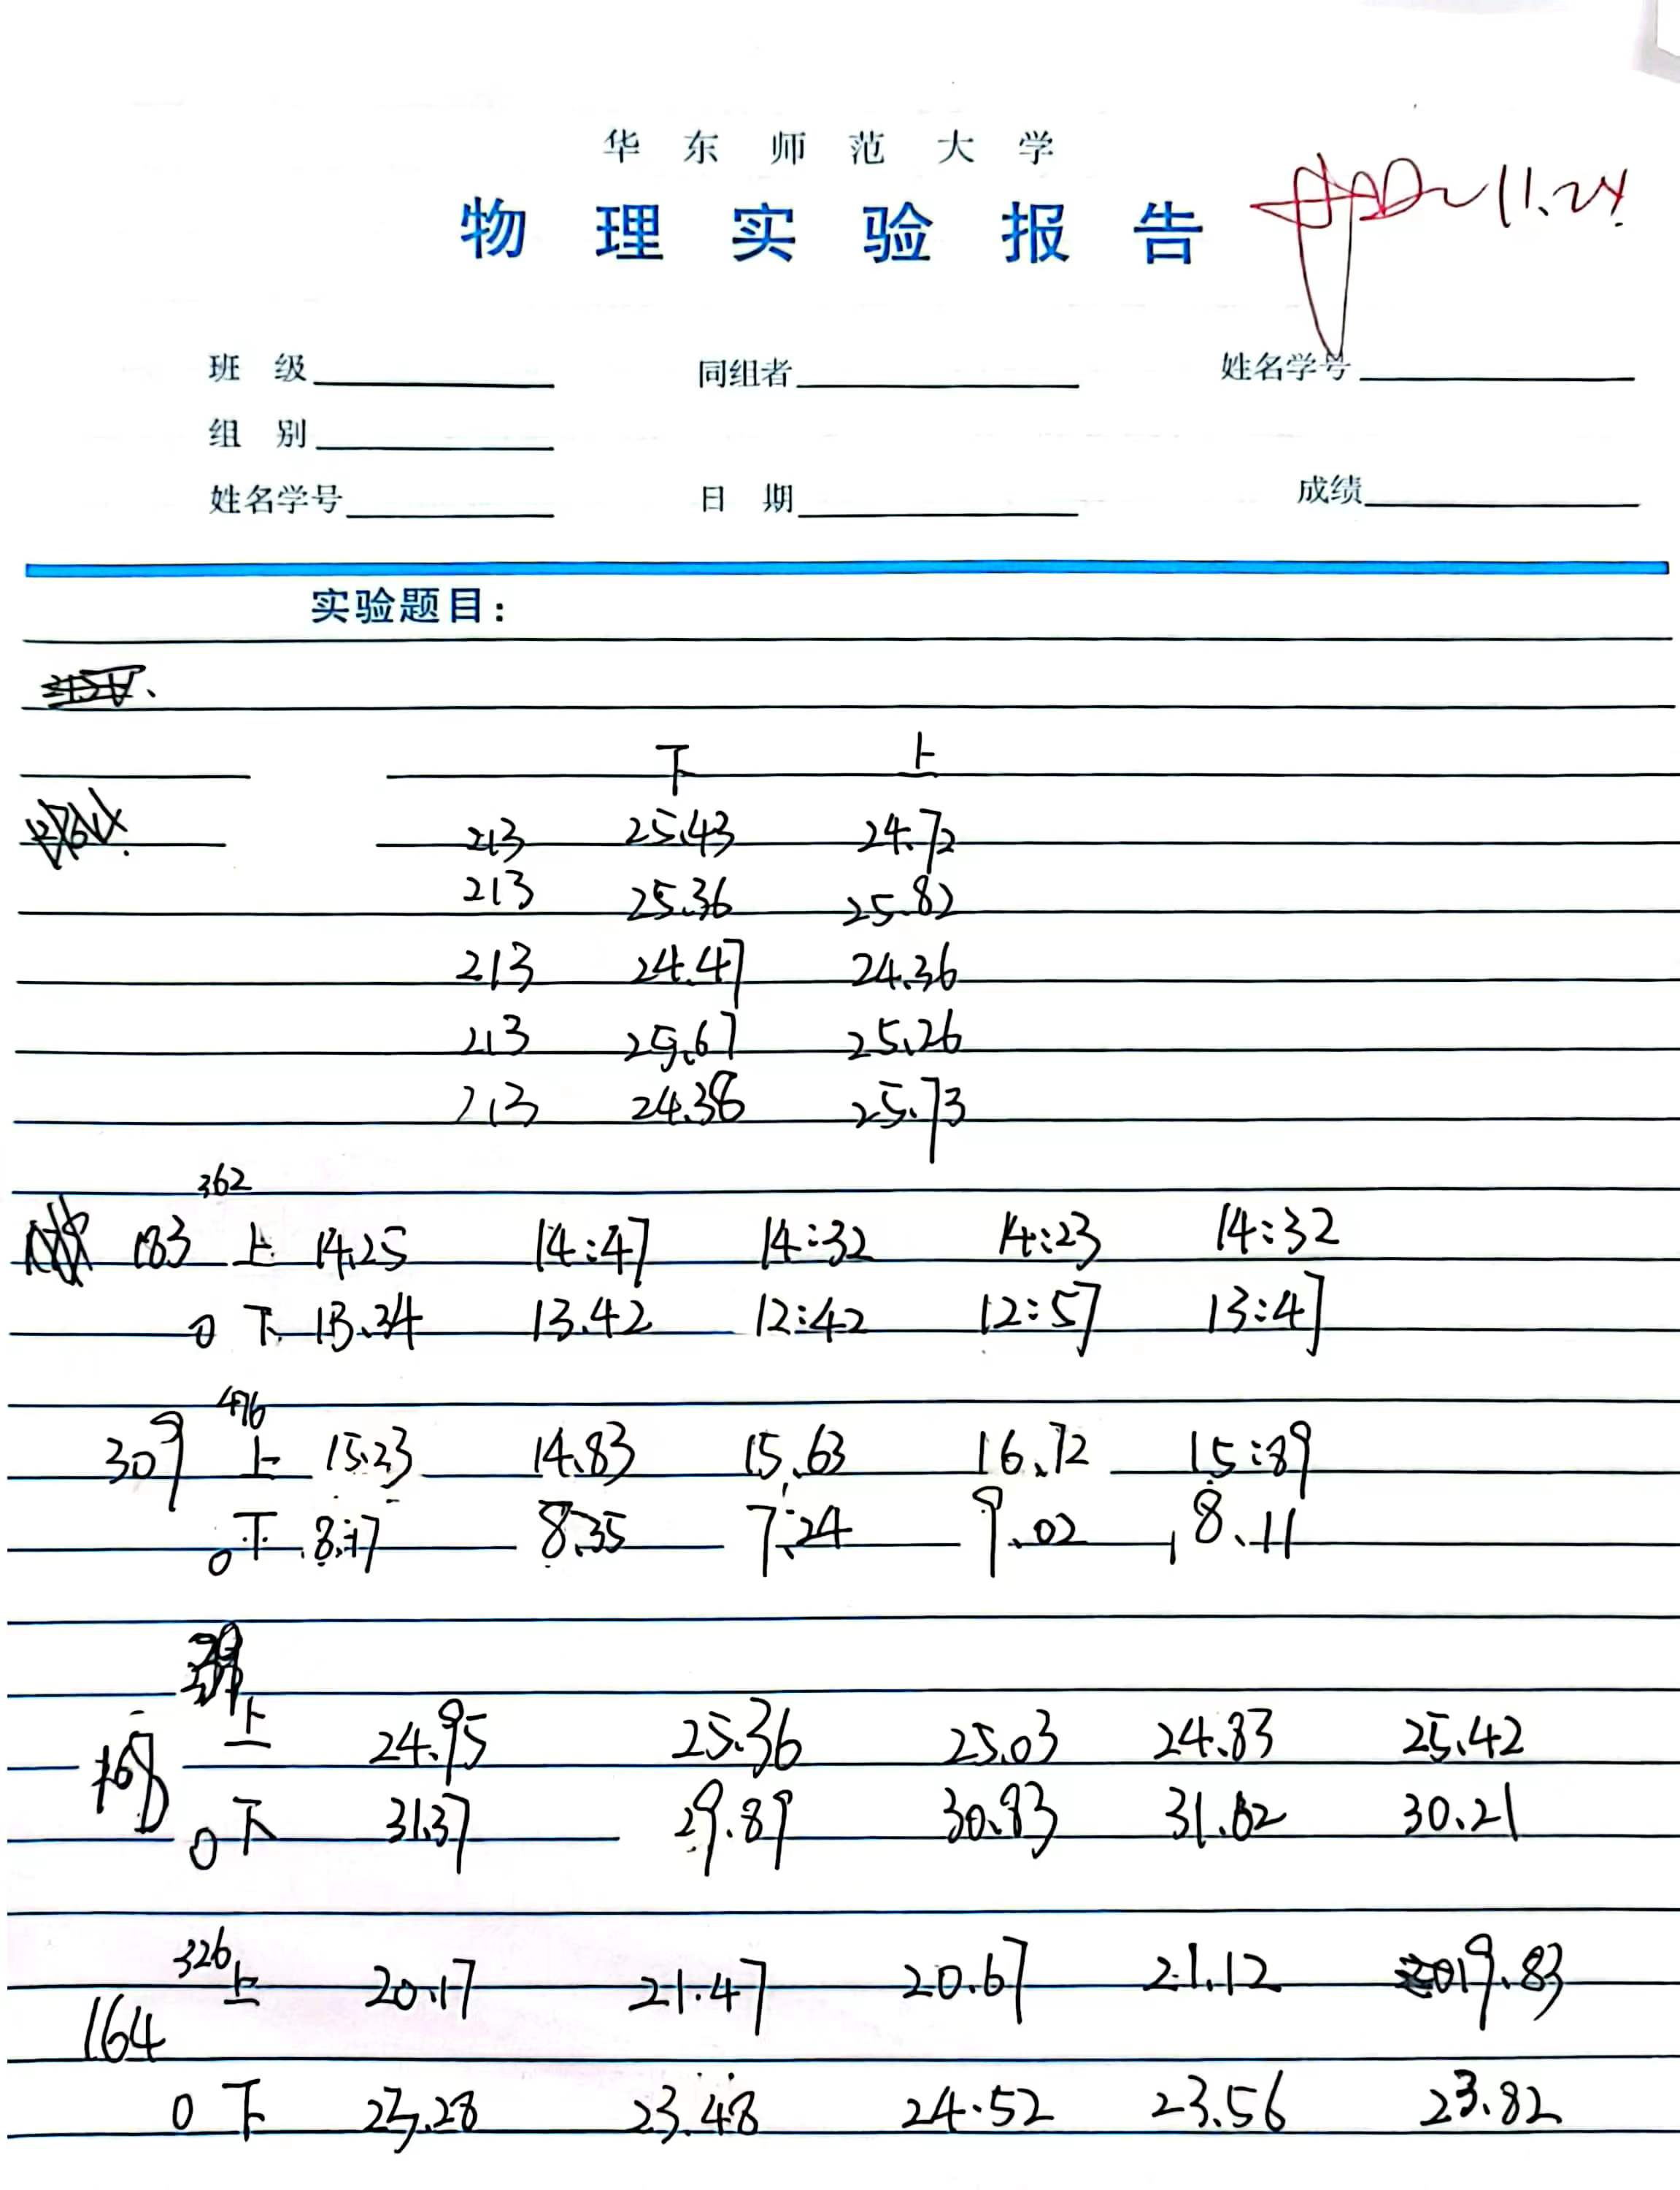
\includegraphics[width=0.9\textwidth,height=0.8\textheight]{yuanshishujv.jpg}
  \caption{实验原始数据1}
\end{figure}
\newpage


\section{实验数据处理}
  \subsection{原始数据及使用的常数展示}
  以下是使用对原始数据的整理和计算所用到的常数的展示。

  \begin{figure}[H]
    \centering
    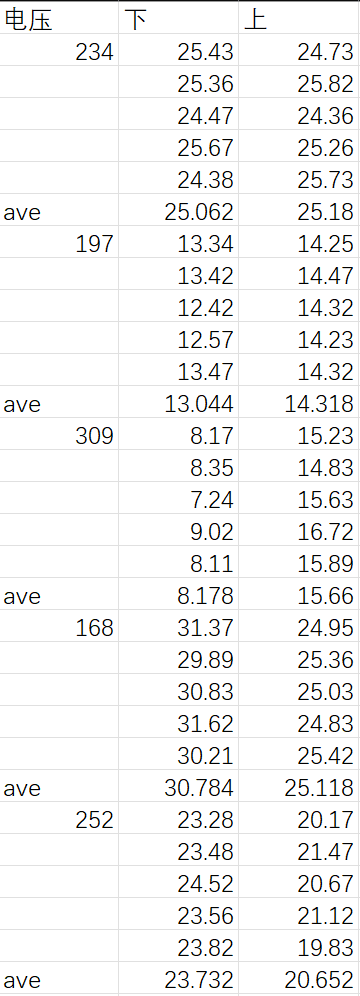
\includegraphics[width=0.5\textwidth,height=0.7\textheight]{shijianshujv.png}
    \caption{实验得到数据}\label{shiyanshujv}
  \end{figure}
  \newpage

  \begin{figure}[H]
    \begin{minipage}[t]{0.4\textwidth}
      \centering
      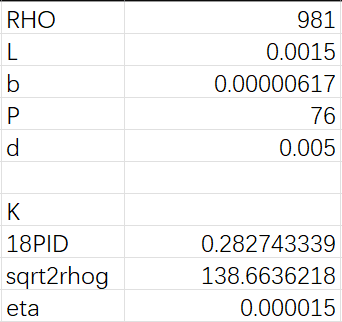
\includegraphics[width=\linewidth]{changshu.png}
      \caption{所使用的常数}\label{changshu}
    \end{minipage}%
    \hfill
    \begin{minipage}[t]{0.6\textwidth}
      实验所使用的常数和实验的数据如图\ref{shiyanshujv}和\ref{changshu}所示。
    \end{minipage}
  \end{figure}

  最终数据中还需要计算常数a和常数K,这两个数据和测量的结果有关,但是在计算中作为常数。
  所以计算两个常数,使用的实验数据是每组实验得到的平均值,最终得到的结果如图
  \ref{consta}和\ref{constk}所示。

  \begin{figure}[H]
    \centering
    \begin{minipage}{0.45\textwidth}
      \centering
      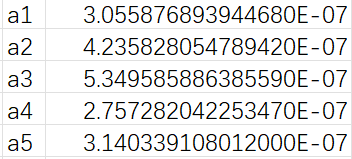
\includegraphics[width=\linewidth]{consta.png}
      \caption{常数a计算}\label{consta}
    \end{minipage}%
    \hfill
    \begin{minipage}{0.45\textwidth}
      \centering
      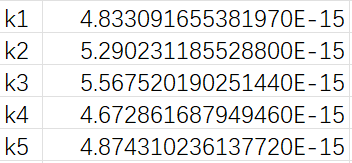
\includegraphics[width=\linewidth]{constk.png}
      \caption{常数K计算}\label{constk}
    \end{minipage}
    \vspace{1em} % 垂直间距
  \end{figure}




  
  \subsection{最大公约数法}
  最大公约数法的结果展示如图\ref{zhijiefa}所示。

  \begin{figure}[H]
    \centering
    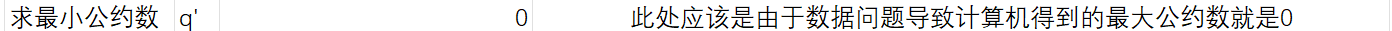
\includegraphics[height=0.03\textwidth,width=1\textwidth]{zhijiefa.png}
    \caption{最大公约数法结果展示}\label{zhijiefa}
  \end{figure}

  从结果中发现,如果通过计算机计算得到的结果是0,原因是实验测得的数据并不是标准的元电荷带电量的整数倍。
  所以直接通过计算机计算将无法通过最大公约数法得到e的值的近似值大小。
  
  \subsection{倒过来验证法}
  倒过来验证法得到的结果展示如图\ref{fanqiufa}所示。

  \begin{figure}[H]
    \centering
    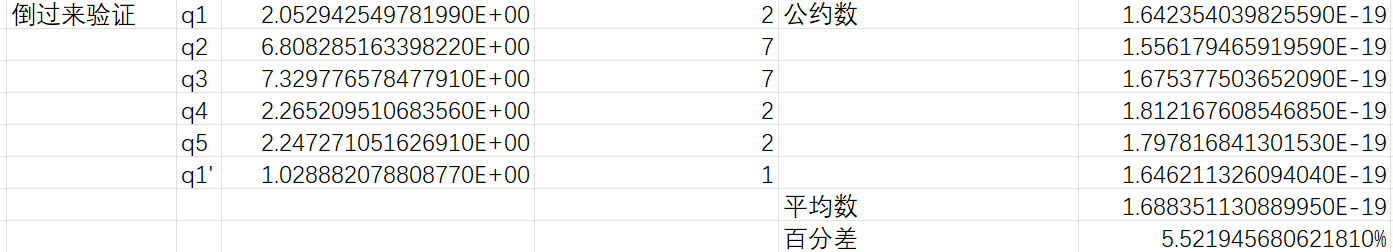
\includegraphics[height=0.25\textwidth,width=1\textwidth]{fanqiufa.png}
    \caption{倒过来验证法结果展示}\label{fanqiufa}
  \end{figure}

  从倒过来验证法中可以看到最终得到的元电荷的大小和理论值之间的百分差在5\%上下,结果还是较为准确的。
  因为在这个过程中是用已知理论值反过来去求的。

  \subsection{作图法}
  作图法得到的结果展示如图\ref{zuotufa}所示。

  \begin{figure}[H]
    \centering
    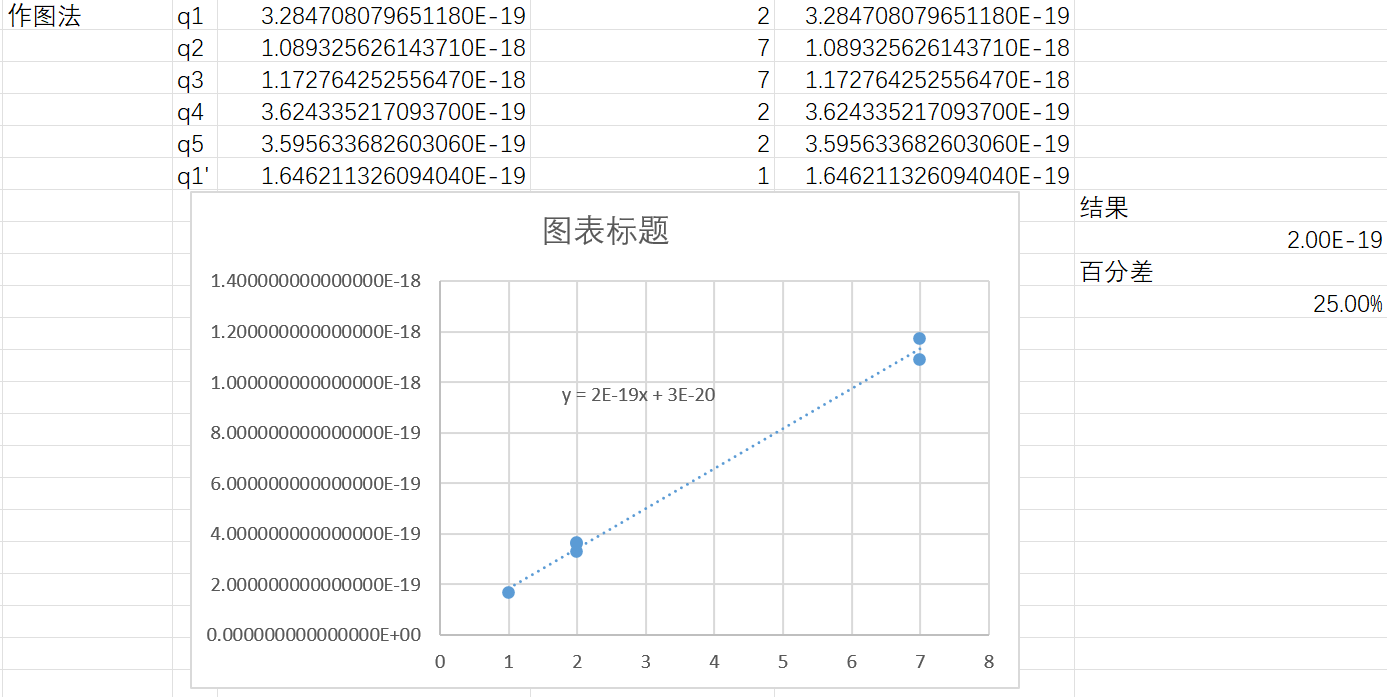
\includegraphics[height=0.5\textwidth,width=1\textwidth]{zuotufa.png}
    \caption{作图法结果展示}\label{zuotufa}
  \end{figure}

  从作图法中可以看到最终得到的元电荷的大小和理论值之间的百分差在25\%上下,结果偏差还是较大的。
  在寻找符合条件的整数的时候选择的是使用GeoGraphic进行处理并寻找的。最后直线是在整数和测得的电荷量
  的图上进行拟合后得到的直线的斜率。误差也较大。GeoGraphic的图像如图\ref{geotu}

  \begin{figure}[H]
    \centering
    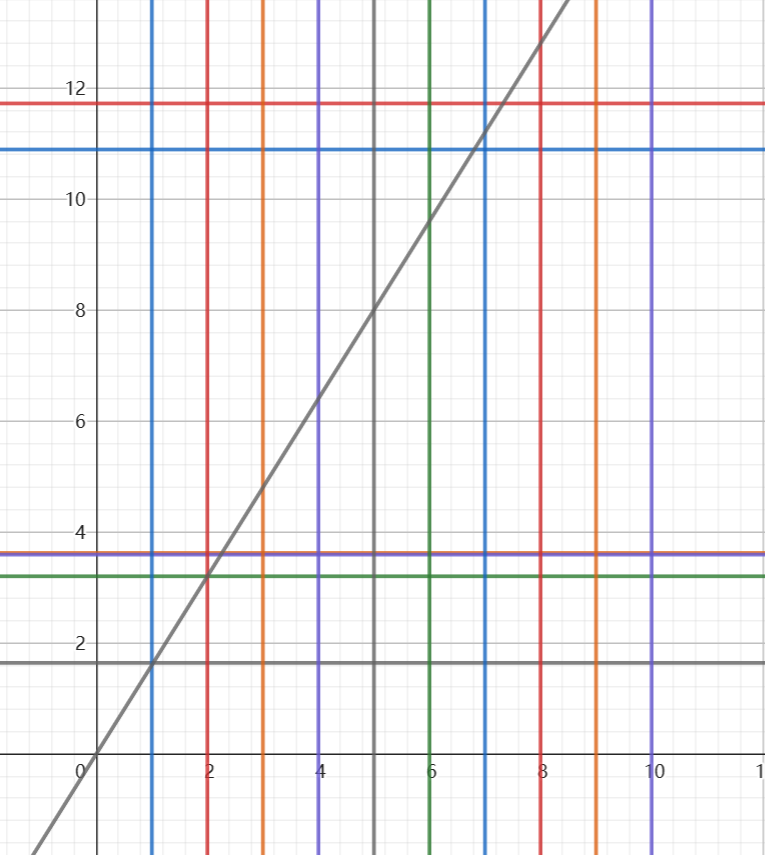
\includegraphics[height=0.5\textwidth,width=0.6\textwidth]{geotu.png}
    \caption{作图法结果展示}\label{geotu}
  \end{figure}

\section{思考题}
  \subsection{思考题一}
  对实验可能产生影响的因素主要有
  油滴的质量和半径、空气阻力、电场的强度、环境温度和湿度、光学系统的精度、电荷的分布和偏离。
  当然,操作者的技术也是主要影响因素。
  \subsection{思考题二}
  让极板平行的方法有:使用水平仪、利用水平线或激光、测量两侧高度。

  如果平行极板不水平,可能会对密立根油滴实验的结果产生一些影响:
  电场非均匀、测量误差、不稳定性,最终导致实验的测量产生误差的错误。

\section{实验中个人的思考与感想}
  \subsection{对于实验个人观点}
  实验非常简单,只要喷油加调节加观察就能得到实验结果。但是实验往往在第一步喷油就结束了。
  想要找到一个符合调节,平衡电压在200v左右,下落时间在20s左右的油滴真的非常困难。而且
  挥发现象在我的实验仪器上非常明显,就会导致最终测试的时候非常容易出现还在调试平衡电压,准备测试了,
  油滴开始扩散挥发原来越模糊。

  总之实验非常需要耐心。但是原理上并不是非常难懂,主要就是一个受力情况的分析。
  \subsection{实验中的总结}
  实验通过测量油滴平衡电压和下降时间计算油滴的受力最终得到油滴所带电荷量。再通过油滴电荷量的
  多个数据求元电荷的大小。

  实验的两种测量方法动态法似乎能够更加准确一些。最终得到的数据的处理也使用了三种不同的方法。
  
  其中直接求最大公约数由于数据并不是准确的理论值,所以寻找比较麻烦,而其他两种中,倒过来计算明显准确很多,
  但是这样和研究目的不符合,变成验证元电荷带电量了。而最后一种作图法得到的数据还是有不少偏差的。
\end{document}
